\chapterimage{Client.jpg} % Chapter heading image

\chapter{System Installation}\index{installation}
\label{sec:SystemInstall}

This chapter explains how to perform a dataClay installation. First, we briefly describe the dataClay architecture for the better understanding of its different components and their interactions. Thereafter, we show how to deploy a minimum dataClay installation based on Dockers\index{dockers}, and how to extrapolate this basic setup to more complex scenarios.

In case you have some other needs not addressed in this chapter, please contact us by email:

\texttt{\href{mailto:support-dataclay@bsc.es}{support-dataclay@bsc.es}}



\section{dataClay architecture}
The architecture of dataClay is composed by two main components: the Logic Module\index{logic module} and the Data Service\index{data service}. The Logic Module is a central repository that handles object metadata and management information. The Data Service is a distributed object store that handles object persistence and execution requests.

\begin{figure}[h]
\centering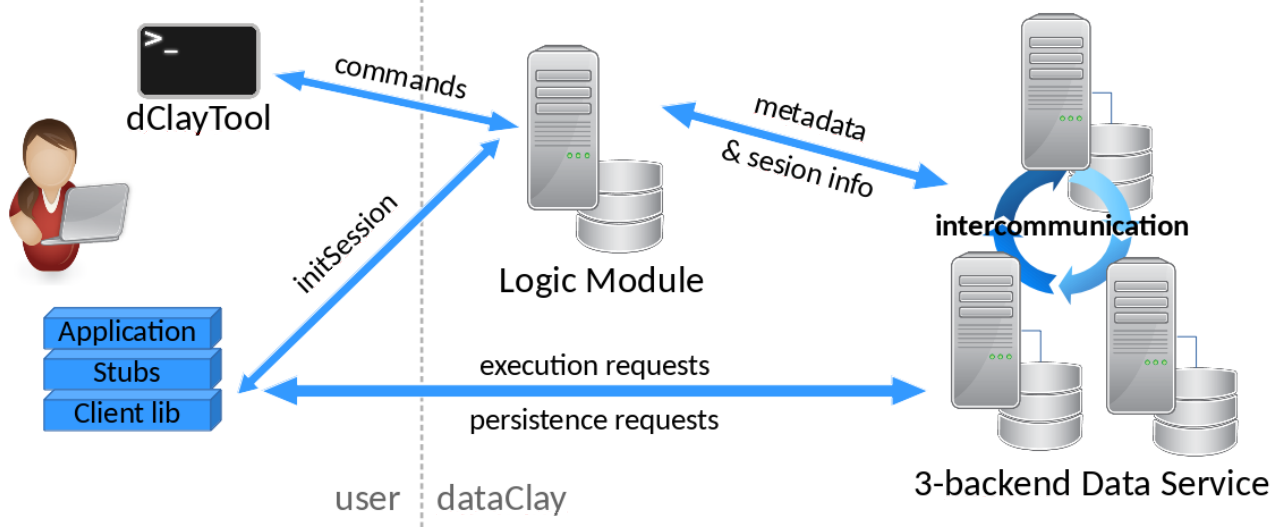
\includegraphics[scale=0.4]{Installation/dataClayOverview}
\caption{dataClay overview}
\label{fig:dataClayOverview}
\end{figure}

\subsection{Logic Module}\index{logic module}
The Logic Module is a unique centralized component that keeps track of every object metadata such as: its unique identifier, (replica) locations, and the dataset it is associated with. 

In addition, the Logic Module is in charge of management info, comprising: accounting, namespaces and datasets, permissions (contracts) and registered class models. That is, the information that can be registered in the system using the \textit{dClayTool} as shown in section \ref{sec:dClayTool}.

Furthermore, the Logic Module is the entry point for any user application, which must authenticate in the system to create a working session and gain permission to interact with the components of the Data Service.

\subsection{Data Service}\index{data service}\index{backend}
\label{sec:DataService}
The Data Service is deployed as a set of multiple backends. Any of these backends handles a subset of objects as well as the execution requests aiming to them. This means that every backend has an \textit{Execution Environment} for all supported languages (currently Java and Python) and an associated \textit{Storage System} to handle object persistence. In the case of Python, where multi-threading cannot be managed as Java does, it is possible to deploy multiple \textit{Execution Environments} sharing a single \textit{Storage System} thus enabling applications to exploit parallelism.

In order to enable \textit{Execution Environments} to handle any kind of object and execution request, the Logic Module is in charge to deploy registered classes to every Data Service backend. In this way, every backend can load stored objects as class instances and execute class methods on them corresponding to upcoming execution requests.

This means that when an application initializes a session with dataClay, it first establishes a connection with the Logic Module and obtains information about the available Data Service backends. At this point, the application is enabled to interact with the Data Service backends through stub classes (retrieved with the \textit{dClayTool}, section \ref{sec:dClayTool}) by submitting execution requests directly to them.



\section{Installation with Docker \index{docker} containers}

Keeping in mind the dataClay architecture, hereafter we show how to deploy a dataClay installation based on Docker \footnote{\url{https://www.docker.com}} containers.

A container image is a lightweight, stand-alone, executable package of a piece of software that includes everything needed to run it: code, runtime, system tools, system libraries, settings. 

In this way, we populate different Docker images corresponding to the main components of the dataClay architecture: the Logic Module and the Data Service. The latter actually comprises one image for each supported language since the corresponding execution requests are handled by separated containers (one per language). 

In order to retrieve these images and orchestrate dataClay services properly, following sections show different scenarios based on the standard \textit{docker-compose}\index{docker-compose} \footnote{\url{https://docs.docker.com/compose/}} tools.

\subsection{Single node installation}
\label{sec:SingleNodeInstall}
This first dataClay installation assumes that all services will run locally on a single node (e.g. your own laptop).

To this end, we will guide you through the installation process by looking at the details of the following \textit{docker-compose} YAML definition:

\begin{tBox}
 \begin{lstlisting}[language=docker-compose-2, frame=none]
version: '2' 
services:
  ####################################
  #  LOGIC MODULE                    #
  ####################################
  lmpostgres:
    image: "bscdataclay/postgres"
    environment:
      - POSTGRES_USER=dataclay
      - POSTGRES_PASSWORD=dataclay
      - POSTGRES_DB=dataclay
    command: -c fsync=off

  logicmodule:
    image: "bscdataclay/logicmodule"
    depends_on:
      - "lmpostgres"
    ports:
      - "11034:11034"
    environment:
      - LOGICMODULE_PORT_TCP=11034
      - POSTGRES_HOST=lmpostgres

  ####################################
  #  BACKEND                         #
  ####################################
  ds1postgres:
    image: "bscdataclay/postgres"
    environment:
      - POSTGRES_USER=dataclay
      - POSTGRES_PASSWORD=dataclay
      - POSTGRES_DB=dataclay
    command: -c fsync=off

  ds1java:
    image: "bscdataclay/dsjava"
    depends_on:
      - "ds1postgres"
      - "logicmodule"
    environment:
      - DATASERVICE_NAME=DS1
      - DATASERVICE_JAVA_PORT_TCP=6866
      - LOGICMODULE_HOST=logicmodule
      - LOGICMODULE_PORT_TCP=11034
      - POSTGRES_HOST=ds1postgres

  ds1pythonee:
    image: "bscdataclay/dspython"
    depends_on:
      - "ds1java"
    environment:
      - DATASERVICE_NAME=DS1
      - DATASERVICE_PYTHON_PORT_TCP=6867
      - LOGICMODULE_HOST=logicmodule
      - LOGICMODULE_PORT_TCP=11034
 \end{lstlisting}
\end{tBox}

Before starting, the first step is to download the required images executing the following command from the directory where this \textit{docker-compose} file resides:
\begin{tBox}
 \begin{bash}
  > docker-compose pull
 \end{bash}
\end{tBox}

At this point, following subsections detail the different parts of the file and which ones can be customized.

\subsubsection{DBMS}
Current version of dataClay might use either PostgreSQL or SQLite for the persistence layer. 

Default DBMS is PostgreSQL which is executed in dedicated containers to serve the Logic Module (\textit{lmpostgres}) and the Data Service (\textit{ds1postgres}). Furthermore, a default user, password and database names are populated to guarantee that PostgreSQL is configured properly.

It is also possible to tune PostgreSQL by passing extra arguments through the \textit{command} subsection. In this case, the \textit{fsync} attribute is deactivated for performance purposes, but you can delete it or activate it if you prefer synchronous updates.

On the other hand, SQLite is deployed as a library so it is already installed in both Logic Module and Data Service images. In this case, we can simplify docker-compose files removing \textit{*postgres} containers, but we have to customize a bit the default configuration of dataClay. Section~\ref{sec:SQLiteConf} shows how to set this up.


\subsubsection{Logic Module}
The \textit{logicmodule}  service corresponds to the Logic Module and refers to its PostgreSQL container through the environment variable \texttt{POSTGRES\_HOST}, by pointing to the host name of its PostgreSQL service: \textit{lmpostgres}.

On the other hand, it is also possible to customize the default Logic Module port, which is currently set to 11034 through environment variable \texttt{LOGICMODULE\_PORT\_TCP} and is mapped to host in \texttt{ports: - ``11034:11034''}. 

In this way, the Logic Module will publish its service at: \texttt{localhost:11034}. In section \ref{sec:ClientConfigFiles} it is described how to define the proper configuration files for user's applications considering this info.

\subsubsection{Data Service Backend - Java}
The \textit{ds1java}  service corresponds to the Java container of the Data Service Backend, and refers to its PostgreSQL container through the environment variable \texttt{POSTGRES\_HOST} by pointing to the host name of its PostgreSQL service: \textit{ds1postgres}.

Every Data Service backend is tagged with a name so containers for all supported languages can be defined as part of the same backend. This is specially useful to, for instance, define a unique PostgreSQL database shared by different execution environments. In this case, the Java container is configured to be part of the Data Service backend called \textit{DS1} as defined via the \texttt{DATASERVICE\_NAME} variable. Furthermore, it is also necessary to specify the port that will be used to handle Java execution requests: \texttt{DATASERVICE\_JAVA\_PORT\_TCP=6866}.

Finally, we also need to specify the address of the Logic Module to enable this Java container to populate its service. To this end, we use the same variables and values as in the Logic Module service (\textit{logicmodule}): \texttt{LOGICMODULE\_HOST=logicmodule} and \texttt{LOGICMODULE\_PORT\_TCP=11034}.

\subsubsection{Data Service Backend - Python}
The Python container does not require any reference to PostgreSQL because currently all data persistence is handled from Java. Therefore, we only need to attach this container to a Data Service backend with Java support. In this case, we attach the Python container to \textit{DS1} Data Service backend through the \texttt{DATASERVICE\_NAME} variable. Furthermore, it is also necessary to specify the port that will be used to handle Java execution requests: \texttt{DATASERVICE\_PYTHON\_PORT\_TCP=6867}.

Finally, we also need to specify the address of the Logic Module to enable this Python container to populate its service. To this end, we use the same variables and values as in the Logic Module service (\textit{logicmodule}): \texttt{LOGICMODULE\_HOST=logicmodule} and \texttt{LOGICMODULE\_PORT\_TCP=11034}.

As mentioned in previous chapters, dataClay supports both Python 2 and Python 3 applications (and corresponding class models), but all the backends in the system, as well as the clients, should use the same Python major version.

By default, Python images tagged as \textit{latest} are based on Python 3, so we need a slight modification in docker-compose files to execute Python 2 applications. In particular, those containers based on \textit{bscdataclay/dspython} image (i.e. \textit{bscdataclay/dspython:latest}) must be modified to use \textit{bscdataclay/dspython:latest-py2.7} instead as in the example below:

\begin{tBox}
 \begin{lstlisting}[language=docker-compose-2, frame=none]
  ds1pythonee:
    image: "bscdataclay/dspython:latest-py2.7"
    depends_on:
      - "ds1java"
    environment:
      - DATASERVICE_NAME=DS1
      - DATASERVICE_PYTHON_PORT_TCP=6867
      - LOGICMODULE_HOST=logicmodule
      - LOGICMODULE_PORT_TCP=11034
 \end{lstlisting}
\end{tBox}


\subsection{Cluster installation}

If you want to deploy dataClay on a cluster of N nodes, you can create different \textit{docker-compose} files for each node depending on the setup you want.

In this section we describe a setup for a 3 node cluster with 1 node for the Logic Module and 2 nodes for Data Service backends. You can easy extrapolate this scenario to more complex ones, but always keeping in mind the following considerations/constraints for the current version of dataClay:

\begin{enumerate}
 \item The Logic Module is unique in the system. This means that only one of the nodes should have a docker-compose file with the Logic Module section.
 \item In this case, all services must be exposed using ``host'' network mode in order to make them visible and discoverable between different nodes and from the client application.
\end{enumerate}

\subsubsection{Node 1 - Logic Module}

The docker-compose file for the first node defining the Logic Module. Notice that using host network we do not need to map its port and \texttt{POSTGRES\_HOST} variable can be set to \textit{localhost}.

\begin{tBox}
 \begin{lstlisting}[language=docker-compose-2, frame=none]
version: '2'
services:
  lmpostgres:
    image: "bscdataclay/postgres"
    environment:
      - POSTGRES_USER=dataclay
      - POSTGRES_PASSWORD=dataclay
      - POSTGRES_DB=dataclay
    command: -c fsync=off
    network_mode: host

  logicmodule:
    image: "bscdataclay/logicmodule"
    depends_on:
      - "lmpostgres"
    environment:
      - LOGICMODULE_PORT_TCP=11034
      - POSTGRES_HOST=localhost
    network_mode: host
 \end{lstlisting}
\end{tBox}

\subsubsection{Node 2 - Backend 1}

This node runs the Data Service backend \textit{DS1}, as specified through the \texttt{DATASERVICE\_NAME} variable.

In the same way as for the Logic Module, \texttt{POSTGRES\_HOST} can be set to \textit{localhost}.

Notice that the only variable that needs to be manually defined is \texttt{LOGICMODULE\_HOST}, which will be the host name of Node 1 where the Logic Module is deployed.

\begin{tBox}
 \begin{lstlisting}[language=docker-compose-2, frame=none]
version: '2'
services:
  ds1postgres:
    image: "bscdataclay/postgres"
    environment:
      - POSTGRES_USER=dataclay
      - POSTGRES_PASSWORD=dataclay
      - POSTGRES_DB=dataclay
    command: -c fsync=off
    network_mode: host

  ds1java:
    image: "bscdataclay/dsjava"
    depends_on:
      - "ds1postgres"
    environment:
      - DATASERVICE_NAME=DS1
      - DATASERVICE_JAVA_PORT_TCP=6866
      - LOGICMODULE_HOST= #TO BE EDITED
      - LOGICMODULE_PORT_TCP=11034
      - POSTGRES_HOST=localhost
    network_mode: host

  ds1pythonee:
    image: "bscdataclay/dspython"
    depends_on:
      - "ds1java"
    environment:
      - DATASERVICE_NAME=DS1
      - DATASERVICE_PYTHON_PORT_TCP=6867
      - LOGICMODULE_HOST= #TO BE EDITED
      - LOGICMODULE_PORT_TCP=11034
    network_mode: host
 \end{lstlisting}
\end{tBox}

\subsubsection{Node 3 - Backend 2}

Analogously to Node 2, this node runs the Data Service backend \textit{DS2}, as specified through the \texttt{DATASERVICE\_NAME} variable.

In the same way as for the Logic Module, \texttt{POSTGRES\_HOST} can be set to \textit{localhost}.

Finally, the only variable that needs to be manually defined is \texttt{LOGICMODULE\_HOST} with the host name of the Node 1 where Logic Module is deployed.

\begin{tBox}
 \begin{lstlisting}[language=docker-compose-2, frame=none]
version: '2'
services:
  ds2postgres:
    image: "bscdataclay/postgres"
    environment:
      - POSTGRES_USER=dataclay
      - POSTGRES_PASSWORD=dataclay
      - POSTGRES_DB=dataclay
    command: -c fsync=off
    network_mode: host

  ds2java:
    image: "bscdataclay/dsjava"
    depends_on:
      - "ds2postgres"
    environment:
      - DATASERVICE_NAME=DS2
      - DATASERVICE_JAVA_PORT_TCP=6866
      - LOGICMODULE_HOST= #TO BE EDITED
      - LOGICMODULE_PORT_TCP=11034
      - POSTGRES_HOST=localhost
    network_mode: host

  ds2pythonee:
    image: "bscdataclay/dspython"
    depends_on:
      - "ds2java"
    environment:
      - DATASERVICE_NAME=DS2
      - DATASERVICE_PYTHON_PORT_TCP=6867
      - LOGICMODULE_HOST= #TO BE EDITED
      - LOGICMODULE_PORT_TCP=11034
    network_mode: host
 \end{lstlisting}
\end{tBox}



\subsection{Enabling Python parallelism}
\label{sec:PythonParallelism}

In Section~\ref{sec:PythonConsiderationsExecutionEnvironment} we explain that the implementation details of the CPython Global Interpreter Lock forces that only one thread can execute Python code at once. However, and as introduced in Section~\ref{sec:DataService}, we can mitigate this problem by configuring dataClay to deploy multiple Python execution environments (backends) on a single node. The example below shows two Python execution environments that will load/store objects from the same Data Service \textit{DS1} ((\textit{ds1pythonee1, ds1pythonee2}).

\begin{tBox}
 \begin{lstlisting}[language=docker-compose-2, frame=none]
version: '2' 
services:
  ####################################
  #  LOGIC MODULE                    #
  ####################################
  lmpostgres:
    image: "bscdataclay/postgres"
    environment:
      - POSTGRES_USER=dataclay
      - POSTGRES_PASSWORD=dataclay
      - POSTGRES_DB=dataclay
    command: -c fsync=off

  logicmodule:
    image: "bscdataclay/logicmodule"
    depends_on:
      - "lmpostgres"
    ports:
      - "11034:11034"
    environment:
      - LOGICMODULE_PORT_TCP=11034
      - POSTGRES_HOST=lmpostgres

  ####################################
  #  BACKEND                         #
  ####################################
  ds1postgres:
    image: "bscdataclay/postgres"
    environment:
      - POSTGRES_USER=dataclay
      - POSTGRES_PASSWORD=dataclay
      - POSTGRES_DB=dataclay
    command: -c fsync=off

  ds1java:
    image: "bscdataclay/dsjava"
    depends_on:
      - "ds1postgres"
      - "logicmodule"
    environment:
      - DATASERVICE_NAME=DS1
      - DATASERVICE_JAVA_PORT_TCP=6866
      - LOGICMODULE_HOST=logicmodule
      - LOGICMODULE_PORT_TCP=11034
      - POSTGRES_HOST=ds1postgres

  ds1pythonee1:
    image: "bscdataclay/dspython"
    depends_on:
      - "ds1java"
    environment:
      - DATASERVICE_NAME=DS1
      - DATASERVICE_PYTHON_PORT_TCP=6867
      - LOGICMODULE_HOST=logicmodule
      - LOGICMODULE_PORT_TCP=11034
      
  ds1pythonee2:
    image: "bscdataclay/dspython"
    depends_on:
      - "ds1java"
    environment:
      - DATASERVICE_NAME=DS1
      - DATASERVICE_PYTHON_PORT_TCP=6867
      - LOGICMODULE_HOST=logicmodule
      - LOGICMODULE_PORT_TCP=11034
 \end{lstlisting}
\end{tBox}

At this point, check Session~\ref{sec:FullTestOtherExamples} if you want to get introduced on how to exploit parallelism with this kind of configurations.


\subsection{Tuning dataClay}

dataClay allows to tune some specific settings (detailed in next sections) using a property file located on a specific path. 

In the application/client side the default path of this file is \texttt{./cfgfiles/global.properties} and can be also defined via the environment variable \texttt{DATACLAY\_GLOBAL\_CONFIG}.

In the server-side the default path is the same, but following previous examples with Docker containers we must define a \textit{volume} to load it. Given the first docker-compose file for a local installation, and assuming that there is a property file located at \texttt{./cfgfiles/global.properties} (relative to the docker-compose file), the volume can be mounted in a per-service basis as illustrated below:

\begin{tBox}
 \begin{lstlisting}[language=docker-compose-2, frame=none]
version: '2' 
services:
  ####################################
  #  LOGIC MODULE                    #
  ####################################
  lmpostgres:
    image: "bscdataclay/postgres"
    environment:
      - POSTGRES_USER=dataclay
      - POSTGRES_PASSWORD=dataclay
      - POSTGRES_DB=dataclay
    command: -c fsync=off

  logicmodule:
    image: "bscdataclay/logicmodule"
    depends_on:
      - "lmpostgres"
    ports:
      - "11034:11034"
    environment:
      - LOGICMODULE_PORT_TCP=11034
      - POSTGRES_HOST=lmpostgres
    volumes:
      - ./cfgfiles/global.properties:/usr/src/dataclay/cfgfiles/global.properties

  ####################################
  #  BACKEND                         #
  ####################################
  ds1postgres:
    image: "bscdataclay/postgres"
    environment:
      - POSTGRES_USER=dataclay
      - POSTGRES_PASSWORD=dataclay
      - POSTGRES_DB=dataclay
    command: -c fsync=off

  ds1java:
    image: "bscdataclay/dsjava"
    depends_on:
      - "ds1postgres"
      - "logicmodule"
    environment:
      - DATASERVICE_NAME=DS1
      - DATASERVICE_JAVA_PORT_TCP=6866
      - LOGICMODULE_HOST=logicmodule
      - LOGICMODULE_PORT_TCP=11034
      - POSTGRES_HOST=ds1postgres
    volumes:
      - ./cfgfiles/global.properties:/usr/src/dataclay/cfgfiles/global.properties

  ds1pythonee:
    image: "bscdataclay/dspython"
    depends_on:
      - "ds1java"
    environment:
      - DATASERVICE_NAME=DS1
      - DATASERVICE_PYTHON_PORT_TCP=6867
      - LOGICMODULE_HOST=logicmodule
      - LOGICMODULE_PORT_TCP=11034     
    volumes:
      - ./cfgfiles/global.properties:/usr/src/dataclay/cfgfiles/global.properties
 \end{lstlisting}
\end{tBox}

\subsubsection{SQLite}
\label{sec:SQLiteConf}

As mentioned in previous sections, dataClay can be configured to use SQLite instead of PostgreSQL. If this is the case, the following flags must be present in \texttt{./cfgfiles/global.properties} to configure Logic Module and Data Service persistence layer respectively:

\begin{itemize}
 \item \begin{verbatim} DB_HANDLER_TYPE_FOR_LOGICMODULE=SQLITE \end{verbatim}
 \item \begin{verbatim} DB_HANDLER_TYPE_FOR_DATASERVICES=SQLITE \end{verbatim}
\end{itemize}

We can also eliminate all postgres containers and related environment variables from docker-compose files, as shown in the following example based on the single-node scenario described in Section~\ref{sec:SingleNodeInstall}:

\begin{tBox}
 \begin{lstlisting}[language=docker-compose-2, frame=none]
version: '2' 
services:
  ####################################
  #  LOGIC MODULE                    #
  ####################################
  logicmodule:
    image: "bscdataclay/logicmodule"
    ports:
      - "11034:11034"
    environment:
      - LOGICMODULE_PORT_TCP=11034
    volumes:
      - ./cfgfiles/global.properties:/usr/src/dataclay/cfgfiles/global.properties

  ####################################
  #  BACKEND                         #
  ####################################
  ds1java:
    image: "bscdataclay/dsjava"
    depends_on:
      - "logicmodule"
    environment:
      - DATASERVICE_NAME=DS1
      - DATASERVICE_JAVA_PORT_TCP=6866
      - LOGICMODULE_HOST=logicmodule
      - LOGICMODULE_PORT_TCP=11034
    volumes:
      - ./cfgfiles/global.properties:/usr/src/dataclay/cfgfiles/global.properties

  ds1pythonee:
    image: "bscdataclay/dspython"
    depends_on:
      - "ds1java"
    environment:
      - DATASERVICE_NAME=DS1
      - DATASERVICE_PYTHON_PORT_TCP=6867
      - LOGICMODULE_HOST=logicmodule
      - LOGICMODULE_PORT_TCP=11034     
    volumes:
      - ./cfgfiles/global.properties:/usr/src/dataclay/cfgfiles/global.properties
 \end{lstlisting}
\end{tBox}


\subsubsection{Memory Management and Garbage Collection}\index{memory management}\index{garbage collection}

In section \ref{sec:GarbageCollection} we have introduced that dataClay runs some processes to keep memory and disk usage in a healthy state. On the one hand, flushing objects from memory to disk when memory usage reaches a certain threshold. On the other hand, keeping track of reference counters to detect objects that are no longer accessible so they can be removed from the system.

To control the impact of these processes on the system performance, dataClay provides the administrator with the capability to configure the following parameters via \textit{global.properties} file. Notice that time parameters are always expressed in milliseconds.

\begin{table}[H]
\footnotesize
\begin{tBox}
\centering
\begin{tabular}{p{57mm} | p{27mm} |  >{\raggedright\arraybackslash}p{50mm}}
\textbf{property} & \textbf{default value} & \textbf{description} \\
\hline
\verb MEMMGMT_PRESSURE_FRACTION & 0.7 (70\%) & Fraction of memory usage from which to consider that it is under pressure. \\
\hline
\verb MEMMGMT_CHECK_TIME_INTERVAL & 5000 (5 seconds) & Periodicity to check memory usage. \\
\hline
\verb GLOBALGC_CHECK_TIME_INTERVAL & 86400000 (1 day) & Periodicity to check and collect objects from underlying storage. \\
\end{tabular}
\label{table:GarbageCollection}
\end{tBox}
\end{table}

An example of the \textit{global.properties} file with non-default values would be as follows:

\begin{tBox}
 \begin{bash}
MEMMGMT_PRESSURE_FRACTION=0.8
MEMMGMT_CHECK_TIME_INTERVAL=8000
GLOBALGC_CHECK_TIME_INTERVAL=1000000
 \end{bash}
\end{tBox}

\subsubsection{Data Prefetching}\index{prefetching}
\label{sec:prefetchingTuning}
As explained in Section \ref{sec:prefetching}, the user can activate data prefetching in dataClay in order to improve the application performance. In order to do so, the following property should be set to true in the \textit{global.properties} file of both the logic module and data services when dataClay is installed.

\begin{table}[H]
\footnotesize
\begin{tBox}
\centering
\begin{tabular}{p{57mm} | p{27mm} |  >{\raggedright\arraybackslash}p{50mm}}
\textbf{property} & \textbf{default value} & \textbf{description} \\
\hline
\verb PREFETCHING_ENABLED & FALSE & Activate or deactivate prefetching in dataClay. \\
\end{tabular}
\label{table:GarbageCollection}
\end{tBox}
\end{table}

Keep in mind that prefetching should also be activated when registering an application using dataClay tool, as explained in Section \ref{sec:newModel}.